\chapter{Administrateur}
\label{admin}

\section{Presentation de l'interface}
Ci-dessous vous pouvez trouver une présentation de l'interface proposée aux administrateur. Dans un soucis de clarté et pour évité de répéter plusieurs fois la même information, en haut de chaques tableaux présents sur le site vous pouvez noter la présence de cases blanches permettant de filtrer les tableaux avec les informations de votre choix puis appliquer ces filtre en appuyant sur la touche entrée de votre clavier.

Pour supprimer tous les filtres, vous pouvez appuyer sur le symbole marqué d'une croix rouge en haut à droite des différents tableaux.

 
\subsection{Accueil}
\label{aa}
Cette sur cette page que l'administrateur arrive à sa connexion. Depuis ce hub, il est possible d'accéder à la grande majorité des pages importante du site.
 \begin{figure}[H]
 	\centering
 	
 	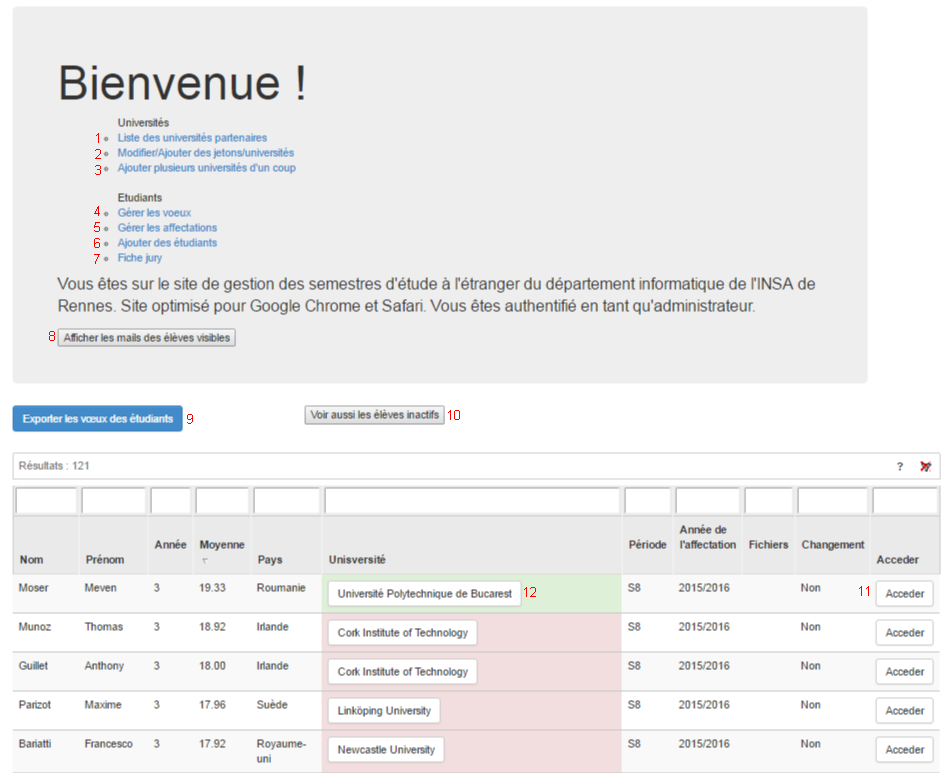
\includegraphics[width=16cm,height=13cm]{Images/Admin/menu_acceuil_admin.png}
 	\caption{Accueil administrateur}
 	
 \end{figure}
 
\begin{enumerate}
\item accès à la liste des étudiant (cf \ref{lua}),
\item accès à la modification des jetons (cf \ref{gua}),
\item accès à la page d'ajout d'universités (cf \ref{pua}),
\item accès à la liste des vœux (cf \ref{lv}),
\item accès à la page permettant d'effectuer l'affectation des élèves (cf \ref{ae}),
\item accès à la page d'ajout des étudiants (cf \ref{aet}),
\item accès à la page de génération de fiches de jury (cf \ref{fj}),
\item ce bouton génère la liste des mails des élèves présent dans le tableau après application des filtres,
\item ce bouton génère un fichier contenant les informations sur les élèves ayant fait des vœux dans l'année courante. Ce fichier CSV peut par la suite être utilisé grâce à excel par exemple,
\item au bout de 5 ans, un élève est considéré comme inactif et n'apparait donc plus dans le tableau. Il est possible de changer cela en cliquant sur ce bouton,
\item ce bouton permet d'accéder à la fiche d'un élève en mode administrateur (cf \ref{ev} , \ref{en} , \ref{ef}),
\item ce bouton permet d'accéder à la fiche d'une université (\ref{fu}).
\end{enumerate}

 
 \subsection{Liste des universités partenaires}
 \label{lua}
 Cette page contient la liste de toutes les universités partenaire de votre département pour lesquelles les élèves peuvent faire des vœux.
 \begin{figure}[H]
 	\centering
 	
 	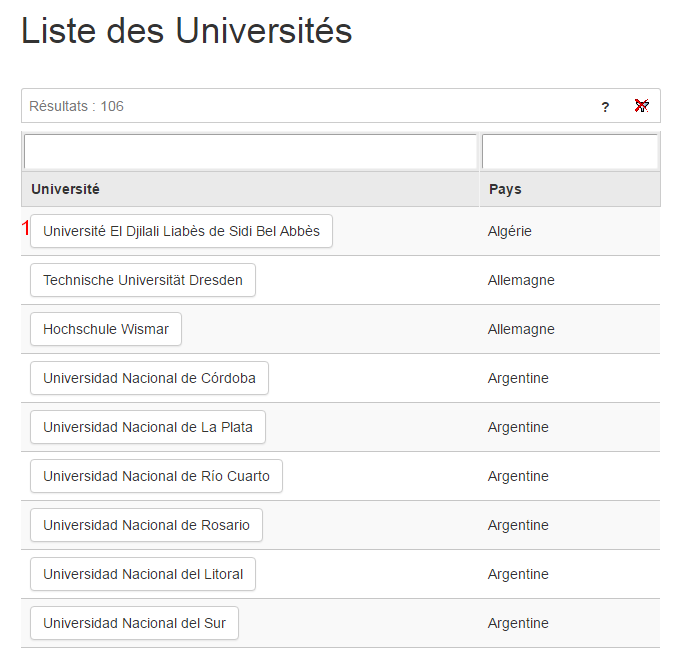
\includegraphics[width=14cm,height=10cm]{Images/Admin/liste_univ_admin.png}
 	\caption{Liste des universités partenaires}
 	
 \end{figure}
 \begin{enumerate}
 \item ce bouton permet d'accéder à la fiche d'une université (cf \ref{fu}).
 \end{enumerate}
 
 \bigbreak\bigbreak\bigbreak
  \subsection{Modifier/Ajouter des jetons/Ajouter des Universités}
  \label{gua}
  Sur cette page il est possible de gérer les jetons disponibles aux élèves de votre département.
  
  \begin{figure}[H]
  	\centering
  	
  	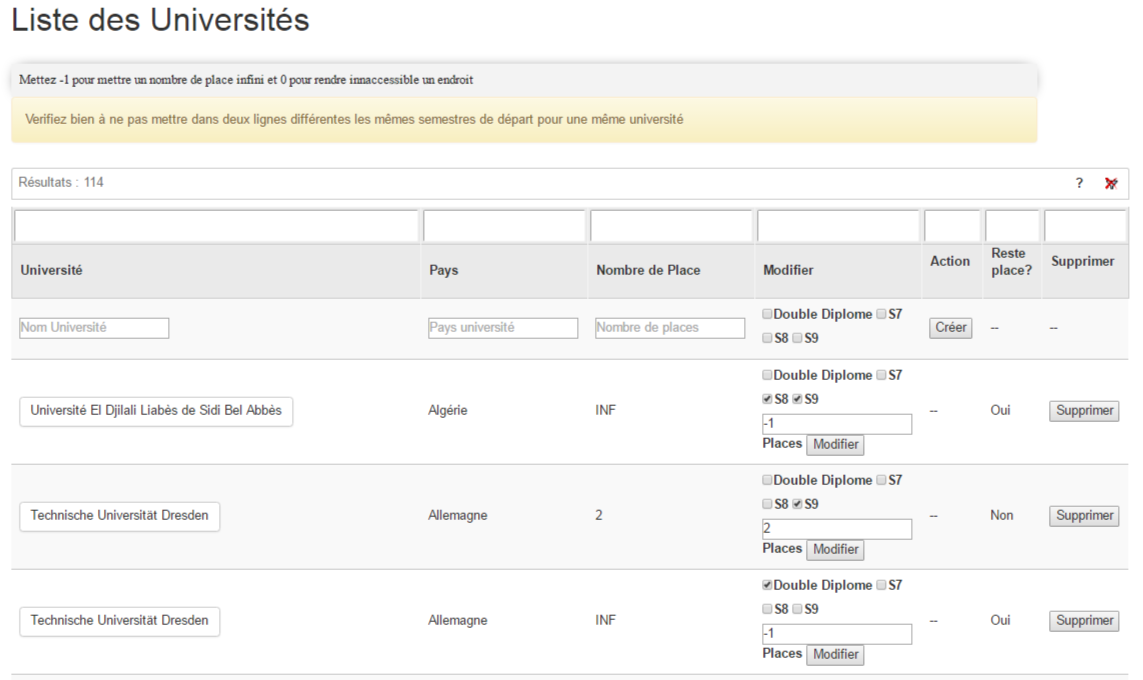
\includegraphics[width=16cm,height=9cm]{Images/Admin/gestion_univ_admin.png}
  	\caption{Modifier/Ajouter des jetons/Ajouter des Universités}
  	
  \end{figure}
   \begin{enumerate}
   	\item cette ligne du tableau permet d'ajouter des nouveaux jetons pour les élèves (cf \ref{cj} pour connaître la procédure à suivre). \att ajouter des jetons à une université qui n'existe pas aura pour effet de l'ajouter dans la base de données,
   	\item ce bouton permet d'accéder à la fiche d'une université (\ref{fu}), 
   	\item ce groupe de champs permet de modifier le nombre de jeton pour une université ainsi que les types de mobilités disponible (cf \ref{mj}),
   	\item ce bouton permet de supprimer les jetons correspondant à la ligne sélectionnée. \att, ce bouton n'entraine pas la suppression totale de l'université mais seulement de ses jetons.
   \end{enumerate}

\newpage
  \subsection{Ajout de plusieurs universités}
  Cette page permet l'ajout de nouvelle universités. l'ajout d'universités se fait par le biais d'un fichier CSV dont le format est précisé sur la page dans la case "Format". Pour plus d'information consultez la section \ref{au}. \att, il est possible d'ajouter une unique université sur la page de gestion des jetons en ajoutant des jetons à une université qui n'existe pas encore.
  \begin{figure}[H]
  	\centering
  	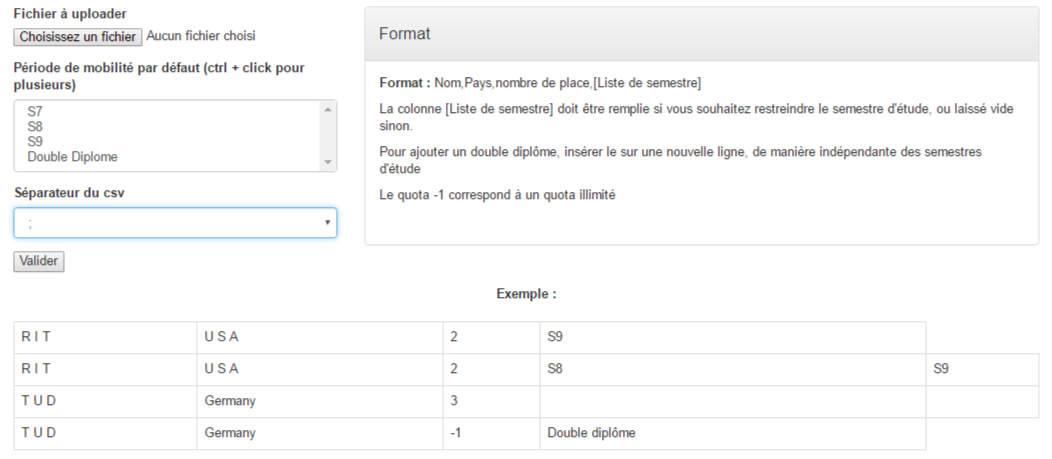
\includegraphics[width=16cm,height=9cm]{Images/Admin/ajout_plusieux_univ_admin.png}
  	\caption{Ajouter plusieurs universités}
  	
  \end{figure}
  \begin{enumerate}
  	\item ce bouton permet d'ouvrir votre explorateur de dossier pour sélectionner le fichier CSV contenant les universités que vous souhaitez ajouter,
  	\item ce menu déroulant permet de sélectionner les mobilités par défaut,
  	\item ce menu déroulant permet de choisir le séparateur utilisé dans votre fichier CSV.\att à bien choisir le CSV correspondant à votre fichier CSV,
  	\item ce bouton permet de valider vos options et valider lancer l'import de vos universités via le CSV.
  \end{enumerate}
  
    \subsection{Fiches de jurys}
    \label{fj}
    \begin{figure}[H]
    	\centering
    	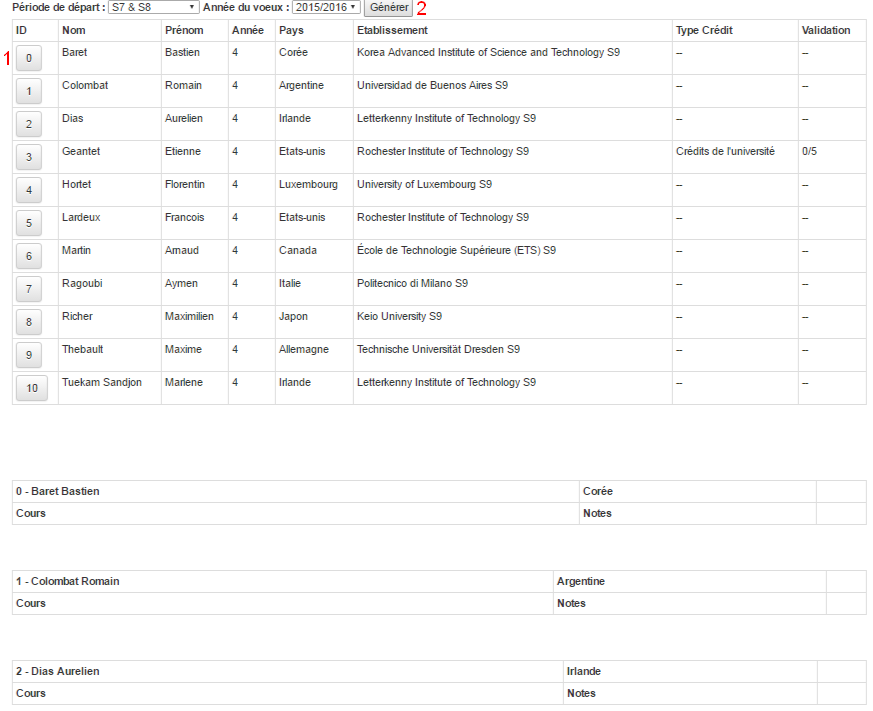
\includegraphics[width=16cm,height=9cm]{Images/Admin/fiche_jury_admin.png}
    	\caption{Fiches de jurys}
    	
    \end{figure}
    \begin{enumerate}
    \item cette ligne permet la génération des fiches de jury. Référez vous à la section \ref{fju},
    \item en cliquant sur ce bouton vous accéder à la page étudiant en mode administrateur (cf \ref{ev}, \ref{en}, \ref{ef}).
    \end{enumerate}
    
    
      
 \subsection{Fiches universités}
 \label{fu}
 Sur cette page sont présente les informations relatives à une universités. On trouve d'abords la liste des départs possibles pour l'universités indépendamment du département. Ensuite le second tableau montre tous les étudiants de votre département ayant fait un vœux pour cette université puis un tableau contenant la liste des tous les élèves déjà partit dans cette université, indépendamment de leur département.
   \begin{figure}[H]
      	\centering
       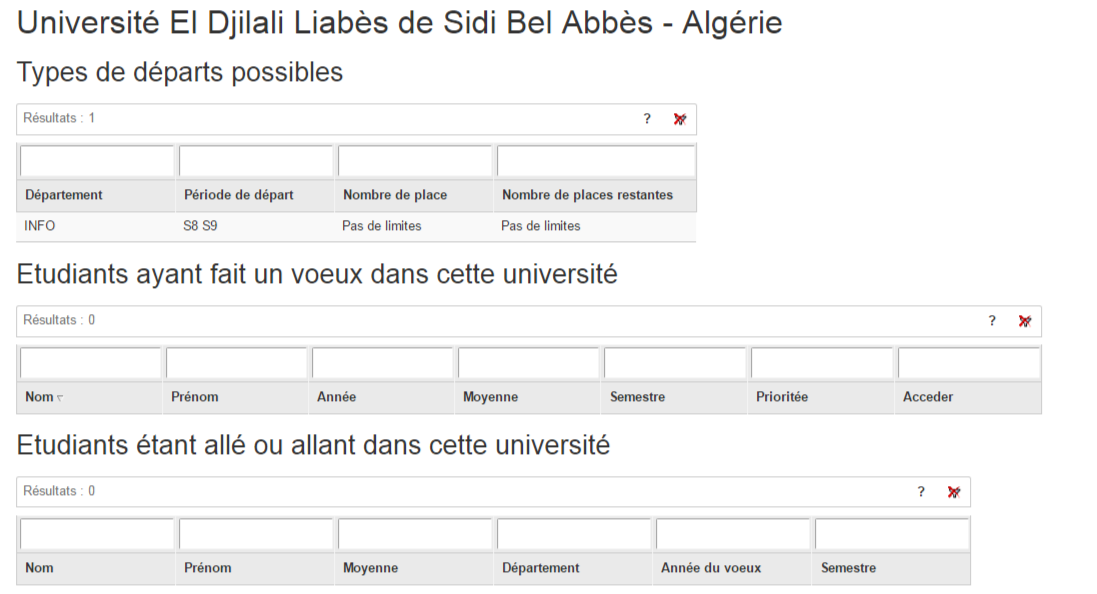
\includegraphics[width=16cm,height=10cm]{Images/Admin/fiche_univ_admin.png}
       \caption{Fiches université}
       
  \end{figure}
  
   \subsection{Liste des vœux}
   \label{lv}
   Cette page résume les vœux de tous les élèves ayant fait des vœux de votre département dans un tableau contenant pour chaque élève la iste de ses trois premiers vœux ainsi que sa destination actuelle (qu'elle soit temporaire ou finale).
   \begin{figure}[H]
   	\centering
   	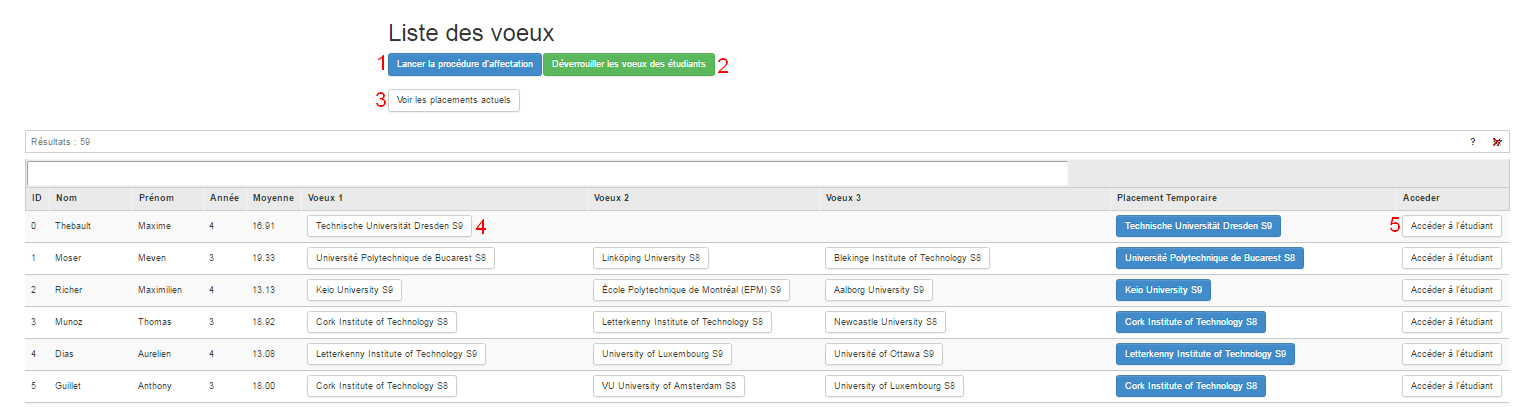
\includegraphics[width=18cm,height=10cm]{Images/Admin/liste_voeux_admin.png}
   	\caption{Liste des vœux} 	
   \end{figure}
   \begin{enumerate}
   	\item en choisissant un des deux algorithmes et en cliquant sur le bouton bleu, vous pouvez lancer une procédure d'affectation. Vous êtes alors redirigé vers la page d'affectation des élèves (cf \ref{ae}). Pour plus d'information sur la procédure d'affectation veuillez vous référer à la section \ref{afv},
   	\item en cliquant sur ce bouton vous êtes redirigé vers la page d'affectation des élèves (cf \ref{ae},)
   	\item en cliquant sur le bouton vert permet de verrouiller ou déverrouiller l'affectation temporaire actuelle de tous les élèves afin qu'il ne change plus si on relance la procédure d'affectation. Pour plus d'information sur la procédure d'affectation veuillez vous référer à la section \ref{afv},
   	\item en cliquant sur ce bouton vous pouvez accéder à la fiche de l'université,
   	\item en cliquant sur ce bouton vous pouvez accéder à la fiche de l'élève correspondant à la ligne du bouton (cf \ref{ev}, \ref{en}, \ref{ef})..
	\end{enumerate}
   
    \subsection{Affectation des élèves}
    \label{ae}
    \begin{figure}[H]
    	\centering
    	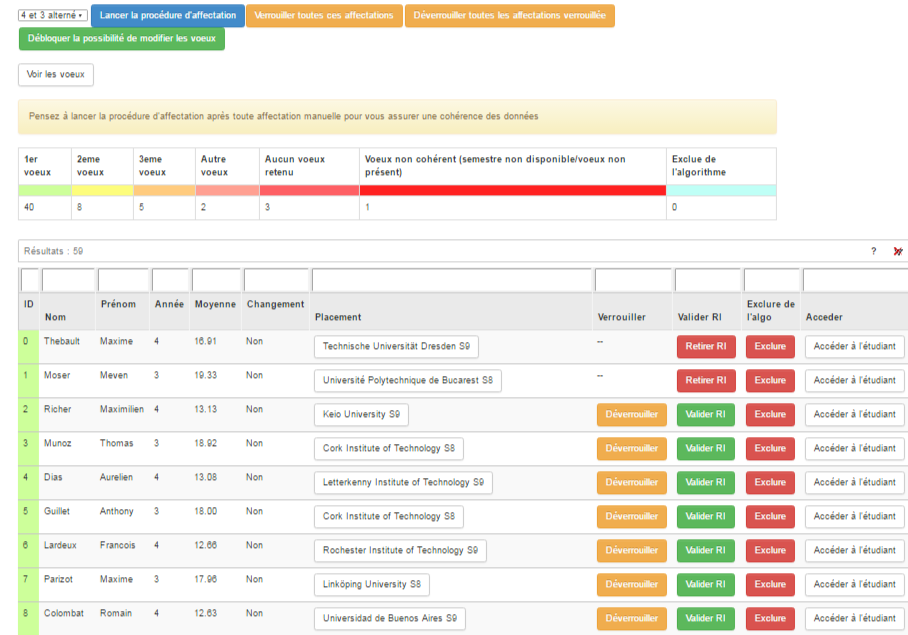
\includegraphics[width=16cm,height=14cm]{Images/Admin/moulinette_admin.png}
    	\caption{Affectation des élèves}
    	
    \end{figure}
             \begin{enumerate}
             	\item en choisissant un des deux algorithmes et en cliquant sur le bouton bleu, vous pouvez lancer une procédure d'affectation. Pour plus d'information sur la procédure d'affectation veuillez vous référer à la section \ref{afv},
             	\item en cliquant sur ce bouton vous pouvez permettre aux élève de faire des vœux ou alors les empêcher de faire des vœux. \att , bien que ce ne soit pas obligatoire, il est conseillé de bloquer la possibilité de vœux avant de lancer les phases d'affectations.
             	\item en cliquant sur ce bouton vous êtes redirigé vers la page de liste des vœux (cf \ref{lv}),
             	\item en cliquant sur ce bouton vous verrouillez tous les élèves ayant fait des vœux afin que leurs vœux ne changent pas à la prochaine affectation. Pour plus d'information sur la procédure d'affectation veuillez vous référer à la section \ref{afv}, 
             	\item en cliquant sur ce bouton vous déverrouillez tous les élèves ayant fait des vœux afin que leurs vœux changent à la prochaine affectation. Pour plus d'information sur la procédure d'affectation veuillez vous référer à la section \ref{afv}, 
             	\item ce tableau exprime à chaque itérations de l'algorithme les statistiques d'affectations,
             	\item en cliquant sur un université vous pouvez accéder à la fiche de l'université (cf \ref{fu}), 
             	\item en cliquant sur ce bouton vous pouvez verrouiller ou déverrouiller la destination d'un élève afin qu'elle soit ou non modifier lors de la procédure d'affectation. Pour plus d'information sur la procédure d'affectation veuillez vous référer à la section \ref{afv},
             	\item ce bouton permet de valider définitivement un élève à sa destination lors de la commission RI. En cas d'erreur il est possible d'invalider un élève en cliquant sur le nouveau bouton "Retirer RI"
             	\item en cliquant sur ce bouton, l'élève voit l'ensemble de ses vœux supprimés et ne peux alors plus partir. néanmoins il reste présent dans la liste des élève et est pris en compte lors de l'algorithme. Pour plus d'information sur la procédure d'affectation veuillez vous référer à la section \ref{afv},
			   	\item en cliquant sur ce bouton vous pouvez accéder à la fiche de l'élève correspondant à la ligne du bouton (cf \ref{ev}, \ref{en}, \ref{ef}).
             \end{enumerate}
    
         \subsection{Page étudiant : Vœux}
         \label{ev}
         \begin{figure}[H]
         	\centering
         	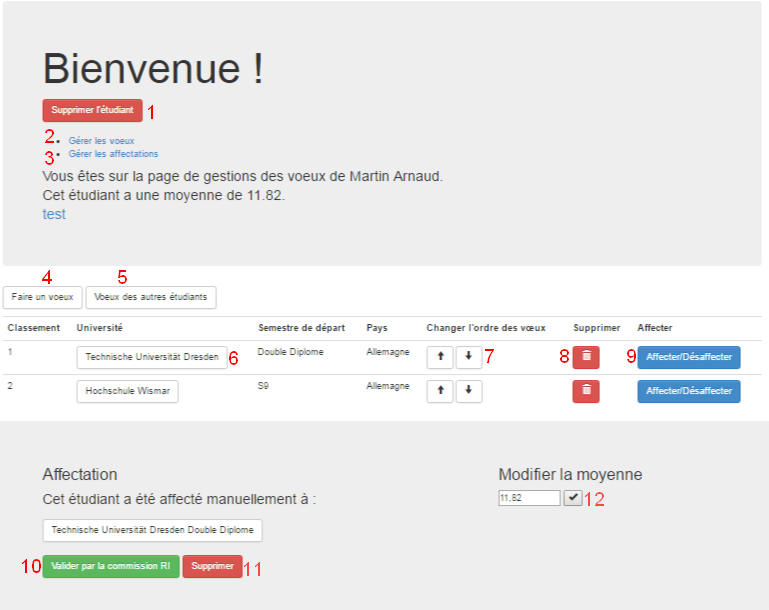
\includegraphics[width=16cm,height=12cm]{Images/Admin/page_etud_admin.png}
         	\caption{Page étudiant : Vœux}
         	
         \end{figure}
                      \begin{enumerate}
                      	\item \att ce bouton supprime définitivement un élève de la base de donnée,
                      	\item ce bouton redirige vers la page de gestion des voeux (cf \ref{lv}),
                      	\item ce bouton redirige vers la page d'affectation (cf \ref{ae}),
                      	\item accès à la liste des universités dans laquelle les élèves sélectionnent leurs vœux (cf \ref{listuniv}),
                     	\item lien vers la liste des étudiants de votre département avec leurs vœux ordonnés,
                      	\item lien vers l'université,
                      	\item flèches permettant de changer l'ordre d'un vœux (monter ou descendre l'ordre de priorité du vœux).
                      	\item cliquez sur ce bouton pour supprimer cette destination de la liste de vos vœux, 
                      	\item ce bouton verrouille ou déverrouille le vœux de l'étudiant afin que celui-ci ne bouge plus lors de la phase d'affectation. Pour plus d'information sur la procédure d'affectation veuillez vous référer à la section \ref{afv},
                      	\item ce bouton permet de valider directement l'affectation de l'élève définitivement, lui permettant ainsi de déposer des contrats d'études. Pour plus d'information sur la procédure d'affectation veuillez vous référer à la section \ref{afv},
                      	\item en cliquant sur ce bouton, l'élève voit l'ensemble de ses vœux supprimés et ne peux alors plus partir. néanmoins il reste présent dans la liste des élève et est pris en compte lors de l'algorithme. Pour plus d'information sur la procédure d'affectation veuillez vous référer à la section \ref{afv},
                      	\item en replissant le champs avec une nouvelle valeur et en cliquant sur le bouton à droite, vous pouvez modifier la note de l'élève.
                      \end{enumerate}

         
    
     \subsection{Page étudiant : Contrat d'étude et notes}
     \label{en}
     \begin{figure}[H]
     	\centering
     	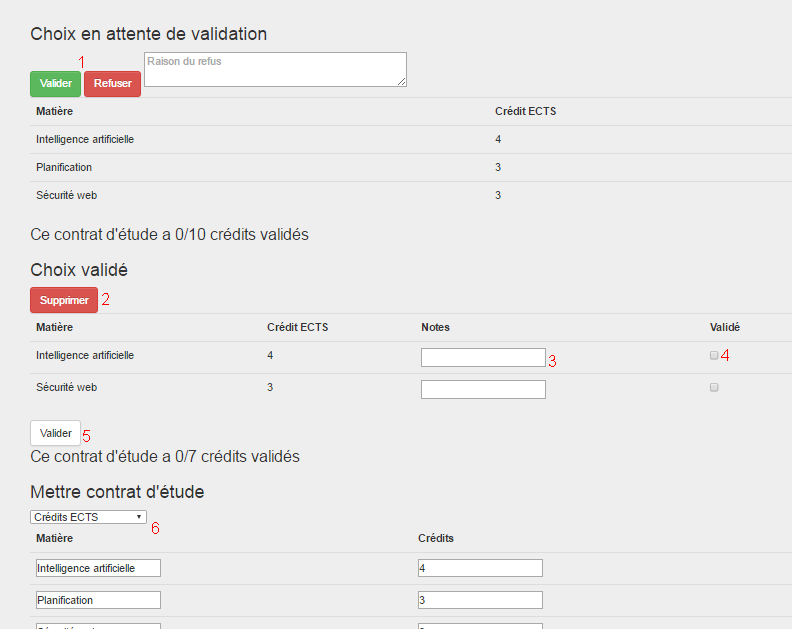
\includegraphics[width=16cm,height=12cm]{Images/Admin/note_admin.png}
     	\caption{Page étudiant : Contrat d'étude et notes}
     	
     \end{figure}
     \begin{enumerate}
     	\item lorsque un élève dépose un contrat d'étude, vous pouvez le valider ou l'invalider en cliquant sur le bouton correspondant. En cas de refus, vous pouvez écrire une raison du refus dans le champs a droite avant de cliquer sur le bouton,
     	\item en cliquant sur ce bouton vous pouvez supprimer un contrat d'étude auparavant validé 
     	\item dans cette case vous pouvez rentrer manuellement les notes de l'élève,
     	\item en cochant cette case, vous assurez que la note obtenue par l'élève permet de valider cette matière pour les fiches de jury,
     	\item cliquez sur ce bouton pour valider les changements apportez aux notes de l'élève,
     	\item dans cette section vous pouvez entrer manuellement un contrat d'étude pour l'élève et le valider directement.
     \end{enumerate}
     
     
          \subsection{Page étudiant : Dépôt de fichier}
          \label{ef}
          \begin{figure}[H]
          	\centering
          	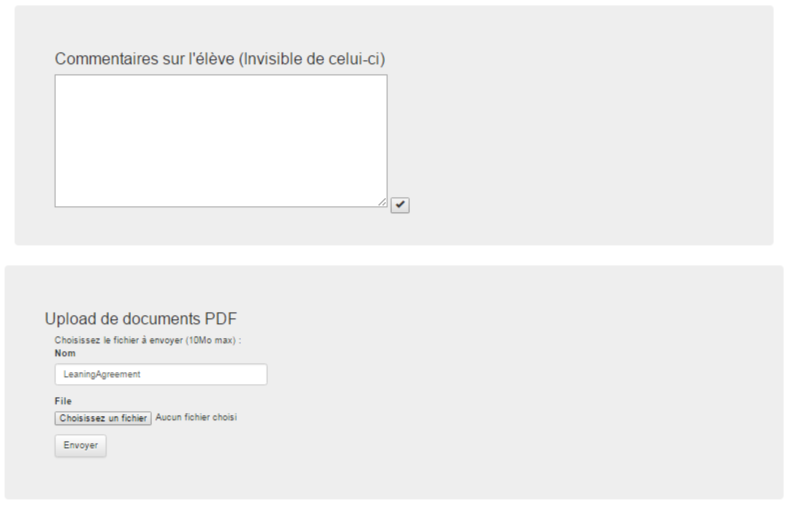
\includegraphics[width=12cm,height=7cm]{Images/Admin/ajout_fichier_admin.png}
          	\caption{Page étudiant : Dépôt de fichier}
          	
          \end{figure}
           \begin{enumerate}
           	\item dans ce champs, vous devez écrire le nom que vous voulez donner au fichier que vous allez déposer sur le site,
           	\item en cliquant sur ce bouton vous ouvrez votre explorateur de fichier pour sélectionner le fichier à déposer
           	\item en cliquant sur ce bouton vous déposer le fichier sur le site.
           \end{enumerate}
          
          \subsection{Ajout d'étudiants}
          \label{aet}
          \begin{figure}[H]
          	\centering
          	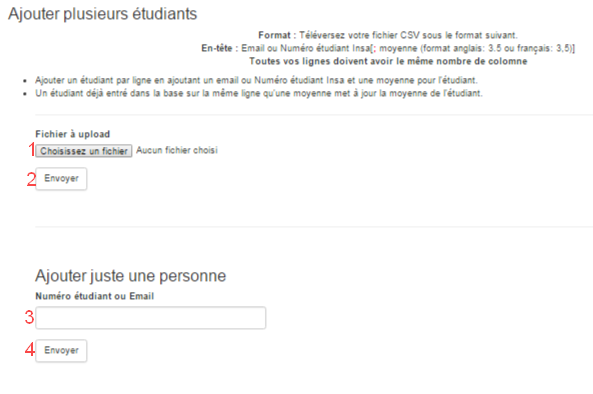
\includegraphics[width=14cm,height=10cm]{Images/Admin/ajout_etud_admin.png}
          	\caption{Ajout d'étudiants}
          	
          \end{figure}
          \begin{enumerate}
          	\item en cliquant sur ce bouton vous ouvrez votre explorateur de fichier pour sélectionner le fichier CSV contenant la liste des élèves à ajouter. Pour plus d'information sur l'ajout de plusieurs élèves veuillez vous référer à la section \ref{ael}
          	\item en cliquant sur ce bouton vous valider l'import du CSV et ajouter la liste des élèves dans la base de données.
          	\item dans cette case vous pouvez entrer le numéro d'étudiant ou l'adresse mail INSA de ce dernier pour l'ajouter à la base de données
          	\item cliquez sur ce bouton pour que l'action d'ajouter un élève soit prise en compte.
          \end{enumerate}
               
        


\section{Gestion des universités}

\subsection{Voir la fiche résumé des universités}

Depuis la page d'accueil \ref{aa} cliquez sur le lien "Liste des universités partenaire". Une fois sur cette page, il vous suffit de cliquer sur le nom de l'université de votre choix pour arriver sur sa page personnelle.
 
\subsection{Modifier les jetons existant d'une université}
\label{mj}
Depuis la page d'accueil \ref{aa} cliquez sur le lien "Modifier/Ajouter des jetons/universités". Vous arrivez sur une page contenant une table avec la liste des jetons associés à une universités pour les semestres cochés. A droite de chaque université, est présente une case "Modifier" dans laquelle vous pouvez modifier la liste des départs disponible à cette destination ainsi que le nombre de place disponible.

\smallbreak

Par exemple, pour une université donnée, les cases S8 et S9 cochés la valeur de 2 pour le nombre de jetons signifie qu'il n'y a que deux places disponibles pour les départs S8 et S9 et non pas 2 places pour S8 et deux places pour S9.

\smallbreak

PS: mettre une valeur de -1 comme nombre de place signifie qu'il y a un nombre illimité de place disponibles.

\subsection{Créer des nouveaux jetons pour une universités}
\label{cj}

Depuis la page de modification des universités (cf paragraphe précédent pour atteindre cette page), si vous souhaitez mettre un nombre de jeton différents pour deux mobilités différentes dans une même université, vous devez créer une nouvelle université ayant le même nom que celle déjà existante puis modifier de manière indépendantes les deux universités.

\smallbreak

Cette méthode doit être utilisée si on souhaite donner un nombre de départs indépendants à deux types de mobilités différentes. Il suffit d'ajouter un nouveau groupe de jeton avec le même nom d'université, et de cocher différentes cases.


\subsection{Ajouter plusieurs universités} 
\label{au}

Depuis la page d'accueil \ref{aa} cliquez sur le lien "Ajoutez plusieurs universités d'un coup". Sur cette page, vous devez uploader un fichier CSV ayant le format décrit dans la case "Format". \att le fichier CSV doit être enregistré au format UTF-8 pour que l'import fonctionne correctement). Choisissez le séparateur correspondant à votre fichier CSV puis cliquer sur valider.

\section{ajouter des élèves}
\label{ael}

//////////////////////////////////

\section{Gestion manuelle des vœux des étudiants}

Depuis la page d'accueil \ref{aa} cliquez sur le lien "Gérer les vœux". Vous arrivez sur une page contenant un tableau résumant par élève la liste de ses 3 premiers vœux. Cliquez ensuite sur "Acceder" pour arriver sur la page élève et pouvoir modifier la liste de ses vœux (ajouter, supprimer) et l'ordre de ses vœux à la place de l'élève (cf section choix des destination du chapitre élève).

\section{Fin de la phase de vœux} 

Depuis la page d'accueil \ref{aa} cliquez sur le lien "Gérer les affectations". Cliquez sur le bouton "Bloquer la possibilité de modifier les veux afin que les élèves ne puissent plus modifier ou ajouter de nouveaux vœux.

\section{Affectation des vœux}
\label{afv}

Sur la page de gestion des affectation (cf paragraphe précédent"), tout d'abords //////////////////////////////////////

\section{Liste de mails}

Depuis la page d'accueil \ref{aa}, avec les filtres selectionner la liste des étudiants qui vous intéressent puis cliquer sur "Afficher les mails des élèves visibles". Il vous suffit ensuite de copier la liste obtenue dans le champs destinataire de votre logiciel de mail.

\section{Gestion des contrat d'étude}

\subsection{Accepter contrat d'étude}
Depuis la page d'accueil, cliquez sur le bouton "acceder" de la ligne correspondant à l'élève souhaité. Un fois sur sa page, si l'élève vous a soumis un contrat d'études, vous pouvez soit le valider en cliquant sur la touche "valider", ou alors le refuser en écrivant si vous le souhaiter une raison à votre refus.

\subsection{Rentrer manuellement un contrat d'étude}
Depuis la page d'un élève, vous pouvez ajoutez manuellement un contrat d'étude et le valider directement.

\section{Dépôt de documents}

Depuis la page d'un étudiant, dans la section "Upload de documents, vous pouvez ajouter des fichiers pour l'élève en question. Pour cela, entrez le nom souhaité pour le document puis cliquer sur "choisissez un fichier" et sélectionnez le fichier. Cliquez enfin sur "envoyer" 

\section{Gérer les notes des élèves}

Depuis la page d'accueil (cf \ref{aa}) vous pouvez accéder à la page d'un élève en cliquant sur le bouton "accéder" (cf \ref{aa}-11) pour aller sur la page de l'étudiant (cf \ref{en}). Depuis cette page, si l'élève à auparavant déposé un contrat d'étude qui a été accepté, vous pouvez rentrer manuellement ses notes (cf \ref{en}-3) et cocher la matière validé (cf \ref{en}-4) afin que les crédit apparaissent dans la fiche de jury générée. Enfin, cliquez sur le bouton "Valider" (cf \ref{en}-5) pour enregistrer les modification.


\section{Générer les fiches de jury}
\label{fju}
Depuis la page d'accueil (cf \ref{aa}) vous pouvez accéder à la page de fiches de jury (cf \ref{fj}) en cliquant sur le lien "Fiche de jury" (cf \ref{aa}-7). Depuis cette page il vous suffit de choisir en haut de la page (cf \ref{fj}-2) la période de départ qui vous intéresse, l'année ou les vœux on été fait et cliquer sur générer afin de créer la fiche de jury de l'ensemble des élèves concernés. 


